%% Font size %%
\documentclass[11pt]{article}

%% Load the custom package
\usepackage{Mathdoc}

%% Numéro de séquence %% Titre de la séquence %%
\renewcommand{\centerhead}{Chap. 5 : Nombres relatifs - Repérage dans le plan}

%% Spacing commands %%
\renewcommand{\baselinestretch}{1}
\setlength{\parindent}{0pt}

\begin{document}

% @see : https://coopmaths.fr/alea?uuid=ab968&id=5R12-2&n=1&d=10&s=1&s2=true&s3=5&alea=4lNA&cd=1&cols=2
\begin{exercice}[1][Déterminer les coordonées.]

\begin{multicols}{2}
 \begin{minipage}[t]{\linewidth} Déterminer les coordonnées des points $C$,  $D$,  $E$,  $B$, et $F$.

\medskip
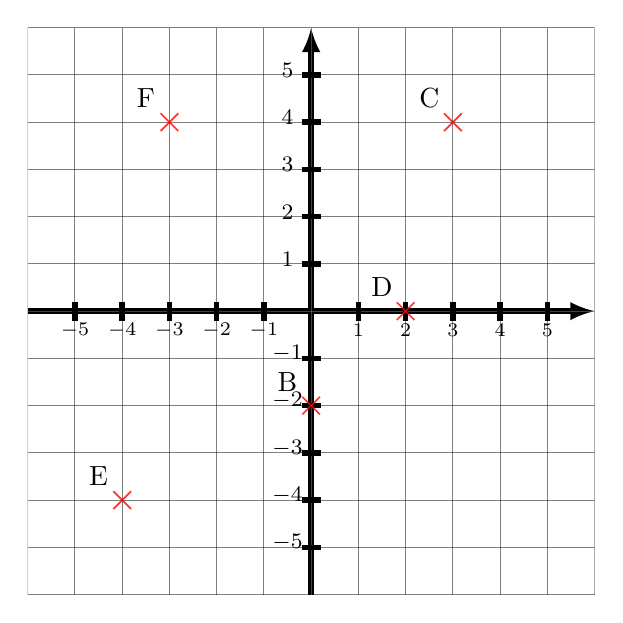
\begin{tikzpicture}[baseline,scale = 0.60]
    \tikzset{
      point/.style={
        thick,
        draw,
        cross out,
        inner sep=0pt,
        minimum width=5pt,
        minimum height=5pt,
      },
    }
    \clip (-6,-6) rectangle (6,6);
    	
	\draw[color ={black},line width = 2,>=latex,->] (-6,0)--(6,0);
	\draw[color ={black},line width = 2,>=latex,->] (0,-6)--(0,6);
	\draw[color ={black},opacity = 0.5] (-6,1)--(6,1);
	\draw[color ={black},opacity = 0.5] (-6,2)--(6,2);
	\draw[color ={black},opacity = 0.5] (-6,3)--(6,3);
	\draw[color ={black},opacity = 0.5] (-6,4)--(6,4);
	\draw[color ={black},opacity = 0.5] (-6,5)--(6,5);
	\draw[color ={black},opacity = 0.5] (-6,6)--(6,6);
	\draw[color ={black},opacity = 0.5] (-6,-1)--(6,-1);
	\draw[color ={black},opacity = 0.5] (-6,-2)--(6,-2);
	\draw[color ={black},opacity = 0.5] (-6,-3)--(6,-3);
	\draw[color ={black},opacity = 0.5] (-6,-4)--(6,-4);
	\draw[color ={black},opacity = 0.5] (-6,-5)--(6,-5);
	\draw[color ={black},opacity = 0.5] (-6,-6)--(6,-6);
	\draw[color ={black},opacity = 0.5] (1,-6)--(1,6);
	\draw[color ={black},opacity = 0.5] (2,-6)--(2,6);
	\draw[color ={black},opacity = 0.5] (3,-6)--(3,6);
	\draw[color ={black},opacity = 0.5] (4,-6)--(4,6);
	\draw[color ={black},opacity = 0.5] (5,-6)--(5,6);
	\draw[color ={black},opacity = 0.5] (6,-6)--(6,6);
	\draw[color ={black},opacity = 0.5] (-1,-6)--(-1,6);
	\draw[color ={black},opacity = 0.5] (-2,-6)--(-2,6);
	\draw[color ={black},opacity = 0.5] (-3,-6)--(-3,6);
	\draw[color ={black},opacity = 0.5] (-4,-6)--(-4,6);
	\draw[color ={black},opacity = 0.5] (-5,-6)--(-5,6);
	\draw[color ={black},opacity = 0.5] (-6,-6)--(-6,6);
	\draw[color ={gray},opacity = 0.3] (-6,0)--(6,0);
	\draw[color ={gray},opacity = 0.3] (-6,0)--(6,0);
	\draw[color ={gray},opacity = 0.3] (0,-6)--(0,6);
	\draw[color ={gray},opacity = 0.3] (0,-6)--(0,6);
	\draw[color ={black},line width = 2] (1,-0.2)--(1,0.2);
	\draw[color ={black},line width = 2] (2,-0.2)--(2,0.2);
	\draw[color ={black},line width = 2] (3,-0.2)--(3,0.2);
	\draw[color ={black},line width = 2] (4,-0.2)--(4,0.2);
	\draw[color ={black},line width = 2] (5,-0.2)--(5,0.2);
	\draw[color ={black},line width = 2] (-1,-0.2)--(-1,0.2);
	\draw[color ={black},line width = 2] (-2,-0.2)--(-2,0.2);
	\draw[color ={black},line width = 2] (-3,-0.2)--(-3,0.2);
	\draw[color ={black},line width = 2] (-4,-0.2)--(-4,0.2);
	\draw[color ={black},line width = 2] (-5,-0.2)--(-5,0.2);
	\draw[color ={black},line width = 2] (-0.2,1)--(0.2,1);
	\draw[color ={black},line width = 2] (-0.2,2)--(0.2,2);
	\draw[color ={black},line width = 2] (-0.2,3)--(0.2,3);
	\draw[color ={black},line width = 2] (-0.2,4)--(0.2,4);
	\draw[color ={black},line width = 2] (-0.2,5)--(0.2,5);
	\draw[color ={black},line width = 2] (-0.2,-1)--(0.2,-1);
	\draw[color ={black},line width = 2] (-0.2,-2)--(0.2,-2);
	\draw[color ={black},line width = 2] (-0.2,-3)--(0.2,-3);
	\draw[color ={black},line width = 2] (-0.2,-4)--(0.2,-4);
	\draw[color ={black},line width = 2] (-0.2,-5)--(0.2,-5);
	\draw (1,-0.4) node[anchor = center] {\scriptsize \color{black}{$1$}};
	\draw (2,-0.4) node[anchor = center] {\scriptsize \color{black}{$2$}};
	\draw (3,-0.4) node[anchor = center] {\scriptsize \color{black}{$3$}};
	\draw (4,-0.4) node[anchor = center] {\scriptsize \color{black}{$4$}};
	\draw (5,-0.4) node[anchor = center] {\scriptsize \color{black}{$5$}};
	\draw (-1,-0.4) node[anchor = center] {\scriptsize \color{black}{$-1$}};
	\draw (-2,-0.4) node[anchor = center] {\scriptsize \color{black}{$-2$}};
	\draw (-3,-0.4) node[anchor = center] {\scriptsize \color{black}{$-3$}};
	\draw (-4,-0.4) node[anchor = center] {\scriptsize \color{black}{$-4$}};
	\draw (-5,-0.4) node[anchor = center] {\scriptsize \color{black}{$-5$}};
	\draw (-0.5,1.1) node[anchor = center] {\footnotesize \color{black}{$1$}};
	\draw (-0.5,2.1) node[anchor = center] {\footnotesize \color{black}{$2$}};
	\draw (-0.5,3.1) node[anchor = center] {\footnotesize \color{black}{$3$}};
	\draw (-0.5,4.1) node[anchor = center] {\footnotesize \color{black}{$4$}};
	\draw (-0.5,5.1) node[anchor = center] {\footnotesize \color{black}{$5$}};
	\draw (-0.5,-0.9) node[anchor = center] {\footnotesize \color{black}{$-1$}};
	\draw (-0.5,-1.9) node[anchor = center] {\footnotesize \color{black}{$-2$}};
	\draw (-0.5,-2.9) node[anchor = center] {\footnotesize \color{black}{$-3$}};
	\draw (-0.5,-3.9) node[anchor = center] {\footnotesize \color{black}{$-4$}};
	\draw (-0.5,-4.9) node[anchor = center] {\footnotesize \color{black}{$-5$}};
	\draw[color ={{red}},line width = 0.625,opacity = 0.8] (2.8125,4.1875)--(3.1875,3.8125);\draw[color ={{red}},line width = 0.625,opacity = 0.8] (2.8125,3.8125)--(3.1875,4.1875);
	\draw [color={black}] (2.5,4.5) node[anchor = center,scale=1, rotate = 0] {C};
	\draw[color ={{red}},line width = 0.625,opacity = 0.8] (1.8125,0.1875)--(2.1875,-0.1875);\draw[color ={{red}},line width = 0.625,opacity = 0.8] (1.8125,-0.1875)--(2.1875,0.1875);
	\draw [color={black}] (1.5,0.5) node[anchor = center,scale=1, rotate = 0] {D};
	\draw[color ={{red}},line width = 0.625,opacity = 0.8] (-4.1875,-3.8125)--(-3.8125,-4.1875);\draw[color ={{red}},line width = 0.625,opacity = 0.8] (-4.1875,-4.1875)--(-3.8125,-3.8125);
	\draw [color={black}] (-4.5,-3.5) node[anchor = center,scale=1, rotate = 0] {E};
	\draw[color ={{red}},line width = 0.625,opacity = 0.8] (-0.1875,-1.8125)--(0.1875,-2.1875);\draw[color ={{red}},line width = 0.625,opacity = 0.8] (-0.1875,-2.1875)--(0.1875,-1.8125);
	\draw [color={black}] (-0.5,-1.5) node[anchor = center,scale=1, rotate = 0] {B};
	\draw[color ={{red}},line width = 0.625,opacity = 0.8] (-3.1875,4.1875)--(-2.8125,3.8125);\draw[color ={{red}},line width = 0.625,opacity = 0.8] (-3.1875,3.8125)--(-2.8125,4.1875);
	\draw [color={black}] (-3.5,4.5) node[anchor = center,scale=1, rotate = 0] {F};

\end{tikzpicture}\\ \end{minipage}

 \begin{minipage}[t]{\linewidth} Déterminer les coordonnées des points $I$,  $M$,  $K$,  $L$, et $J$.

\medskip
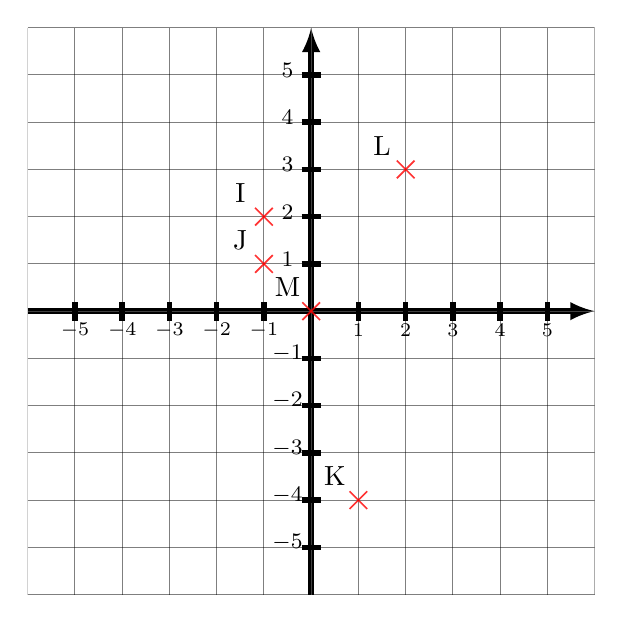
\begin{tikzpicture}[baseline,scale = 0.60]

    \tikzset{
      point/.style={
        thick,
        draw,
        cross out,
        inner sep=0pt,
        minimum width=5pt,
        minimum height=5pt,
      },
    }
    \clip (-6,-6) rectangle (6,6);
    	
	\draw[color ={black},line width = 2,>=latex,->] (-6,0)--(6,0);
	\draw[color ={black},line width = 2,>=latex,->] (0,-6)--(0,6);
	\draw[color ={black},opacity = 0.5] (-6,1)--(6,1);
	\draw[color ={black},opacity = 0.5] (-6,2)--(6,2);
	\draw[color ={black},opacity = 0.5] (-6,3)--(6,3);
	\draw[color ={black},opacity = 0.5] (-6,4)--(6,4);
	\draw[color ={black},opacity = 0.5] (-6,5)--(6,5);
	\draw[color ={black},opacity = 0.5] (-6,6)--(6,6);
	\draw[color ={black},opacity = 0.5] (-6,-1)--(6,-1);
	\draw[color ={black},opacity = 0.5] (-6,-2)--(6,-2);
	\draw[color ={black},opacity = 0.5] (-6,-3)--(6,-3);
	\draw[color ={black},opacity = 0.5] (-6,-4)--(6,-4);
	\draw[color ={black},opacity = 0.5] (-6,-5)--(6,-5);
	\draw[color ={black},opacity = 0.5] (-6,-6)--(6,-6);
	\draw[color ={black},opacity = 0.5] (1,-6)--(1,6);
	\draw[color ={black},opacity = 0.5] (2,-6)--(2,6);
	\draw[color ={black},opacity = 0.5] (3,-6)--(3,6);
	\draw[color ={black},opacity = 0.5] (4,-6)--(4,6);
	\draw[color ={black},opacity = 0.5] (5,-6)--(5,6);
	\draw[color ={black},opacity = 0.5] (6,-6)--(6,6);
	\draw[color ={black},opacity = 0.5] (-1,-6)--(-1,6);
	\draw[color ={black},opacity = 0.5] (-2,-6)--(-2,6);
	\draw[color ={black},opacity = 0.5] (-3,-6)--(-3,6);
	\draw[color ={black},opacity = 0.5] (-4,-6)--(-4,6);
	\draw[color ={black},opacity = 0.5] (-5,-6)--(-5,6);
	\draw[color ={black},opacity = 0.5] (-6,-6)--(-6,6);
	\draw[color ={gray},opacity = 0.3] (-6,0)--(6,0);
	\draw[color ={gray},opacity = 0.3] (-6,0)--(6,0);
	\draw[color ={gray},opacity = 0.3] (0,-6)--(0,6);
	\draw[color ={gray},opacity = 0.3] (0,-6)--(0,6);
	\draw[color ={black},line width = 2] (1,-0.2)--(1,0.2);
	\draw[color ={black},line width = 2] (2,-0.2)--(2,0.2);
	\draw[color ={black},line width = 2] (3,-0.2)--(3,0.2);
	\draw[color ={black},line width = 2] (4,-0.2)--(4,0.2);
	\draw[color ={black},line width = 2] (5,-0.2)--(5,0.2);
	\draw[color ={black},line width = 2] (-1,-0.2)--(-1,0.2);
	\draw[color ={black},line width = 2] (-2,-0.2)--(-2,0.2);
	\draw[color ={black},line width = 2] (-3,-0.2)--(-3,0.2);
	\draw[color ={black},line width = 2] (-4,-0.2)--(-4,0.2);
	\draw[color ={black},line width = 2] (-5,-0.2)--(-5,0.2);
	\draw[color ={black},line width = 2] (-0.2,1)--(0.2,1);
	\draw[color ={black},line width = 2] (-0.2,2)--(0.2,2);
	\draw[color ={black},line width = 2] (-0.2,3)--(0.2,3);
	\draw[color ={black},line width = 2] (-0.2,4)--(0.2,4);
	\draw[color ={black},line width = 2] (-0.2,5)--(0.2,5);
	\draw[color ={black},line width = 2] (-0.2,-1)--(0.2,-1);
	\draw[color ={black},line width = 2] (-0.2,-2)--(0.2,-2);
	\draw[color ={black},line width = 2] (-0.2,-3)--(0.2,-3);
	\draw[color ={black},line width = 2] (-0.2,-4)--(0.2,-4);
	\draw[color ={black},line width = 2] (-0.2,-5)--(0.2,-5);
	\draw (1,-0.4) node[anchor = center] {\scriptsize \color{black}{$1$}};
	\draw (2,-0.4) node[anchor = center] {\scriptsize \color{black}{$2$}};
	\draw (3,-0.4) node[anchor = center] {\scriptsize \color{black}{$3$}};
	\draw (4,-0.4) node[anchor = center] {\scriptsize \color{black}{$4$}};
	\draw (5,-0.4) node[anchor = center] {\scriptsize \color{black}{$5$}};
	\draw (-1,-0.4) node[anchor = center] {\scriptsize \color{black}{$-1$}};
	\draw (-2,-0.4) node[anchor = center] {\scriptsize \color{black}{$-2$}};
	\draw (-3,-0.4) node[anchor = center] {\scriptsize \color{black}{$-3$}};
	\draw (-4,-0.4) node[anchor = center] {\scriptsize \color{black}{$-4$}};
	\draw (-5,-0.4) node[anchor = center] {\scriptsize \color{black}{$-5$}};
	\draw (-0.5,1.1) node[anchor = center] {\footnotesize \color{black}{$1$}};
	\draw (-0.5,2.1) node[anchor = center] {\footnotesize \color{black}{$2$}};
	\draw (-0.5,3.1) node[anchor = center] {\footnotesize \color{black}{$3$}};
	\draw (-0.5,4.1) node[anchor = center] {\footnotesize \color{black}{$4$}};
	\draw (-0.5,5.1) node[anchor = center] {\footnotesize \color{black}{$5$}};
	\draw (-0.5,-0.9) node[anchor = center] {\footnotesize \color{black}{$-1$}};
	\draw (-0.5,-1.9) node[anchor = center] {\footnotesize \color{black}{$-2$}};
	\draw (-0.5,-2.9) node[anchor = center] {\footnotesize \color{black}{$-3$}};
	\draw (-0.5,-3.9) node[anchor = center] {\footnotesize \color{black}{$-4$}};
	\draw (-0.5,-4.9) node[anchor = center] {\footnotesize \color{black}{$-5$}};
	\draw[color ={{red}},line width = 0.625,opacity = 0.8] (-1.1875,2.1875)--(-0.8125,1.8125);\draw[color ={{red}},line width = 0.625,opacity = 0.8] (-1.1875,1.8125)--(-0.8125,2.1875);
	\draw [color={black}] (-1.5,2.5) node[anchor = center,scale=1, rotate = 0] {I};
	\draw[color ={{red}},line width = 0.625,opacity = 0.8] (-0.1875,0.1875)--(0.1875,-0.1875);\draw[color ={{red}},line width = 0.625,opacity = 0.8] (-0.1875,-0.1875)--(0.1875,0.1875);
	\draw [color={black}] (-0.5,0.5) node[anchor = center,scale=1, rotate = 0] {M};
	\draw[color ={{red}},line width = 0.625,opacity = 0.8] (0.8125,-3.8125)--(1.1875,-4.1875);\draw[color ={{red}},line width = 0.625,opacity = 0.8] (0.8125,-4.1875)--(1.1875,-3.8125);
	\draw [color={black}] (0.5,-3.5) node[anchor = center,scale=1, rotate = 0] {K};
	\draw[color ={{red}},line width = 0.625,opacity = 0.8] (1.8125,3.1875)--(2.1875,2.8125);\draw[color ={{red}},line width = 0.625,opacity = 0.8] (1.8125,2.8125)--(2.1875,3.1875);
	\draw [color={black}] (1.5,3.5) node[anchor = center,scale=1, rotate = 0] {L};
	\draw[color ={{red}},line width = 0.625,opacity = 0.8] (-1.1875,1.1875)--(-0.8125,0.8125);\draw[color ={{red}},line width = 0.625,opacity = 0.8] (-1.1875,0.8125)--(-0.8125,1.1875);
	\draw [color={black}] (-1.5,1.5) node[anchor = center,scale=1, rotate = 0] {J};

\end{tikzpicture}\\ \end{minipage}
\end{multicols}
\end{exercice}


\begin{exercice}[2][Déterminer les coordonnées.]
\begin{multicols}{2}
 \begin{minipage}[t]{\linewidth} Déterminer les coordonnées des points $O$,  $N$,  $L$,  $P$, et $M$.

\medskip
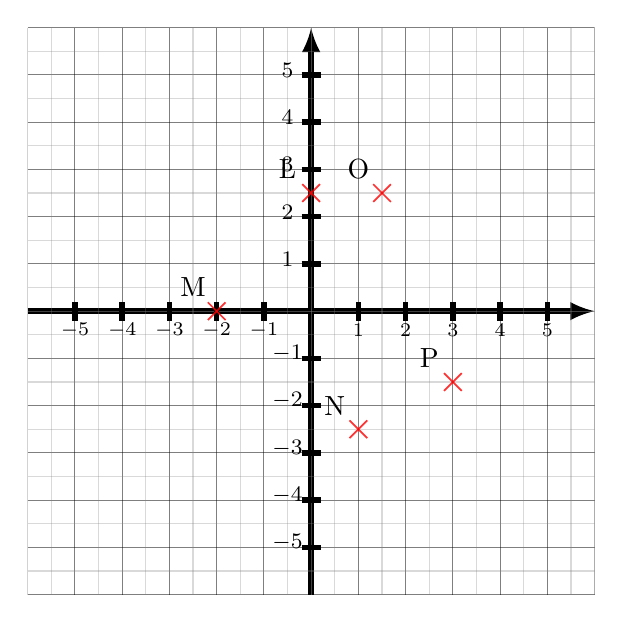
\begin{tikzpicture}[baseline,scale = 0.60]

    \tikzset{
      point/.style={
        thick,
        draw,
        cross out,
        inner sep=0pt,
        minimum width=5pt,
        minimum height=5pt,
      },
    }
    \clip (-6,-6) rectangle (6,6);
    	
	\draw[color ={black},line width = 2,>=latex,->] (-6,0)--(6,0);
	\draw[color ={black},line width = 2,>=latex,->] (0,-6)--(0,6);
	\draw[color ={black},opacity = 0.5] (-6,1)--(6,1);
	\draw[color ={black},opacity = 0.5] (-6,2)--(6,2);
	\draw[color ={black},opacity = 0.5] (-6,3)--(6,3);
	\draw[color ={black},opacity = 0.5] (-6,4)--(6,4);
	\draw[color ={black},opacity = 0.5] (-6,5)--(6,5);
	\draw[color ={black},opacity = 0.5] (-6,6)--(6,6);
	\draw[color ={black},opacity = 0.5] (-6,-1)--(6,-1);
	\draw[color ={black},opacity = 0.5] (-6,-2)--(6,-2);
	\draw[color ={black},opacity = 0.5] (-6,-3)--(6,-3);
	\draw[color ={black},opacity = 0.5] (-6,-4)--(6,-4);
	\draw[color ={black},opacity = 0.5] (-6,-5)--(6,-5);
	\draw[color ={black},opacity = 0.5] (-6,-6)--(6,-6);
	\draw[color ={black},opacity = 0.5] (1,-6)--(1,6);
	\draw[color ={black},opacity = 0.5] (2,-6)--(2,6);
	\draw[color ={black},opacity = 0.5] (3,-6)--(3,6);
	\draw[color ={black},opacity = 0.5] (4,-6)--(4,6);
	\draw[color ={black},opacity = 0.5] (5,-6)--(5,6);
	\draw[color ={black},opacity = 0.5] (6,-6)--(6,6);
	\draw[color ={black},opacity = 0.5] (-1,-6)--(-1,6);
	\draw[color ={black},opacity = 0.5] (-2,-6)--(-2,6);
	\draw[color ={black},opacity = 0.5] (-3,-6)--(-3,6);
	\draw[color ={black},opacity = 0.5] (-4,-6)--(-4,6);
	\draw[color ={black},opacity = 0.5] (-5,-6)--(-5,6);
	\draw[color ={black},opacity = 0.5] (-6,-6)--(-6,6);
	\draw[color ={gray},opacity = 0.3] (-6,0)--(6,0);
	\draw[color ={gray},opacity = 0.3] (-6,0.5)--(6,0.5);
	\draw[color ={gray},opacity = 0.3] (-6,1.5)--(6,1.5);
	\draw[color ={gray},opacity = 0.3] (-6,2.5)--(6,2.5);
	\draw[color ={gray},opacity = 0.3] (-6,3.5)--(6,3.5);
	\draw[color ={gray},opacity = 0.3] (-6,4.5)--(6,4.5);
	\draw[color ={gray},opacity = 0.3] (-6,5.5)--(6,5.5);
	\draw[color ={gray},opacity = 0.3] (-6,0)--(6,0);
	\draw[color ={gray},opacity = 0.3] (-6,-0.5)--(6,-0.5);
	\draw[color ={gray},opacity = 0.3] (-6,-1.5)--(6,-1.5);
	\draw[color ={gray},opacity = 0.3] (-6,-2.5)--(6,-2.5);
	\draw[color ={gray},opacity = 0.3] (-6,-3.5)--(6,-3.5);
	\draw[color ={gray},opacity = 0.3] (-6,-4.5)--(6,-4.5);
	\draw[color ={gray},opacity = 0.3] (-6,-5.5)--(6,-5.5);
	\draw[color ={gray},opacity = 0.3] (0,-6)--(0,6);
	\draw[color ={gray},opacity = 0.3] (0.5,-6)--(0.5,6);
	\draw[color ={gray},opacity = 0.3] (1.5,-6)--(1.5,6);
	\draw[color ={gray},opacity = 0.3] (2.5,-6)--(2.5,6);
	\draw[color ={gray},opacity = 0.3] (3.5,-6)--(3.5,6);
	\draw[color ={gray},opacity = 0.3] (4.5,-6)--(4.5,6);
	\draw[color ={gray},opacity = 0.3] (5.5,-6)--(5.5,6);
	\draw[color ={gray},opacity = 0.3] (0,-6)--(0,6);
	\draw[color ={gray},opacity = 0.3] (-0.5,-6)--(-0.5,6);
	\draw[color ={gray},opacity = 0.3] (-1.5,-6)--(-1.5,6);
	\draw[color ={gray},opacity = 0.3] (-2.5,-6)--(-2.5,6);
	\draw[color ={gray},opacity = 0.3] (-3.5,-6)--(-3.5,6);
	\draw[color ={gray},opacity = 0.3] (-4.5,-6)--(-4.5,6);
	\draw[color ={gray},opacity = 0.3] (-5.5,-6)--(-5.5,6);
	\draw[color ={black},line width = 2] (1,-0.2)--(1,0.2);
	\draw[color ={black},line width = 2] (2,-0.2)--(2,0.2);
	\draw[color ={black},line width = 2] (3,-0.2)--(3,0.2);
	\draw[color ={black},line width = 2] (4,-0.2)--(4,0.2);
	\draw[color ={black},line width = 2] (5,-0.2)--(5,0.2);
	\draw[color ={black},line width = 2] (-1,-0.2)--(-1,0.2);
	\draw[color ={black},line width = 2] (-2,-0.2)--(-2,0.2);
	\draw[color ={black},line width = 2] (-3,-0.2)--(-3,0.2);
	\draw[color ={black},line width = 2] (-4,-0.2)--(-4,0.2);
	\draw[color ={black},line width = 2] (-5,-0.2)--(-5,0.2);
	\draw[color ={black},line width = 2] (-0.2,1)--(0.2,1);
	\draw[color ={black},line width = 2] (-0.2,2)--(0.2,2);
	\draw[color ={black},line width = 2] (-0.2,3)--(0.2,3);
	\draw[color ={black},line width = 2] (-0.2,4)--(0.2,4);
	\draw[color ={black},line width = 2] (-0.2,5)--(0.2,5);
	\draw[color ={black},line width = 2] (-0.2,-1)--(0.2,-1);
	\draw[color ={black},line width = 2] (-0.2,-2)--(0.2,-2);
	\draw[color ={black},line width = 2] (-0.2,-3)--(0.2,-3);
	\draw[color ={black},line width = 2] (-0.2,-4)--(0.2,-4);
	\draw[color ={black},line width = 2] (-0.2,-5)--(0.2,-5);
	\draw (1,-0.4) node[anchor = center] {\scriptsize \color{black}{$1$}};
	\draw (2,-0.4) node[anchor = center] {\scriptsize \color{black}{$2$}};
	\draw (3,-0.4) node[anchor = center] {\scriptsize \color{black}{$3$}};
	\draw (4,-0.4) node[anchor = center] {\scriptsize \color{black}{$4$}};
	\draw (5,-0.4) node[anchor = center] {\scriptsize \color{black}{$5$}};
	\draw (-1,-0.4) node[anchor = center] {\scriptsize \color{black}{$-1$}};
	\draw (-2,-0.4) node[anchor = center] {\scriptsize \color{black}{$-2$}};
	\draw (-3,-0.4) node[anchor = center] {\scriptsize \color{black}{$-3$}};
	\draw (-4,-0.4) node[anchor = center] {\scriptsize \color{black}{$-4$}};
	\draw (-5,-0.4) node[anchor = center] {\scriptsize \color{black}{$-5$}};
	\draw (-0.5,1.1) node[anchor = center] {\footnotesize \color{black}{$1$}};
	\draw (-0.5,2.1) node[anchor = center] {\footnotesize \color{black}{$2$}};
	\draw (-0.5,3.1) node[anchor = center] {\footnotesize \color{black}{$3$}};
	\draw (-0.5,4.1) node[anchor = center] {\footnotesize \color{black}{$4$}};
	\draw (-0.5,5.1) node[anchor = center] {\footnotesize \color{black}{$5$}};
	\draw (-0.5,-0.9) node[anchor = center] {\footnotesize \color{black}{$-1$}};
	\draw (-0.5,-1.9) node[anchor = center] {\footnotesize \color{black}{$-2$}};
	\draw (-0.5,-2.9) node[anchor = center] {\footnotesize \color{black}{$-3$}};
	\draw (-0.5,-3.9) node[anchor = center] {\footnotesize \color{black}{$-4$}};
	\draw (-0.5,-4.9) node[anchor = center] {\footnotesize \color{black}{$-5$}};
	\draw[color ={{red}},line width = 0.625,opacity = 0.8] (1.3125,2.6875)--(1.6875,2.3125);\draw[color ={{red}},line width = 0.625,opacity = 0.8] (1.3125,2.3125)--(1.6875,2.6875);
	\draw [color={black}] (1,3) node[anchor = center,scale=1, rotate = 0] {O};
	\draw[color ={{red}},line width = 0.625,opacity = 0.8] (0.8125,-2.3125)--(1.1875,-2.6875);\draw[color ={{red}},line width = 0.625,opacity = 0.8] (0.8125,-2.6875)--(1.1875,-2.3125);
	\draw [color={black}] (0.5,-2) node[anchor = center,scale=1, rotate = 0] {N};
	\draw[color ={{red}},line width = 0.625,opacity = 0.8] (-0.1875,2.6875)--(0.1875,2.3125);\draw[color ={{red}},line width = 0.625,opacity = 0.8] (-0.1875,2.3125)--(0.1875,2.6875);
	\draw [color={black}] (-0.5,3) node[anchor = center,scale=1, rotate = 0] {L};
	\draw[color ={{red}},line width = 0.625,opacity = 0.8] (2.8125,-1.3125)--(3.1875,-1.6875);\draw[color ={{red}},line width = 0.625,opacity = 0.8] (2.8125,-1.6875)--(3.1875,-1.3125);
	\draw [color={black}] (2.5,-1) node[anchor = center,scale=1, rotate = 0] {P};
	\draw[color ={{red}},line width = 0.625,opacity = 0.8] (-2.1875,0.1875)--(-1.8125,-0.1875);\draw[color ={{red}},line width = 0.625,opacity = 0.8] (-2.1875,-0.1875)--(-1.8125,0.1875);
	\draw [color={black}] (-2.5,0.5) node[anchor = center,scale=1, rotate = 0] {M};

\end{tikzpicture}\\ \end{minipage}

 \begin{minipage}[t]{\linewidth} Déterminer les coordonnées des points $P$,  $T$,  $R$,  $Q$, et $S$.

\medskip
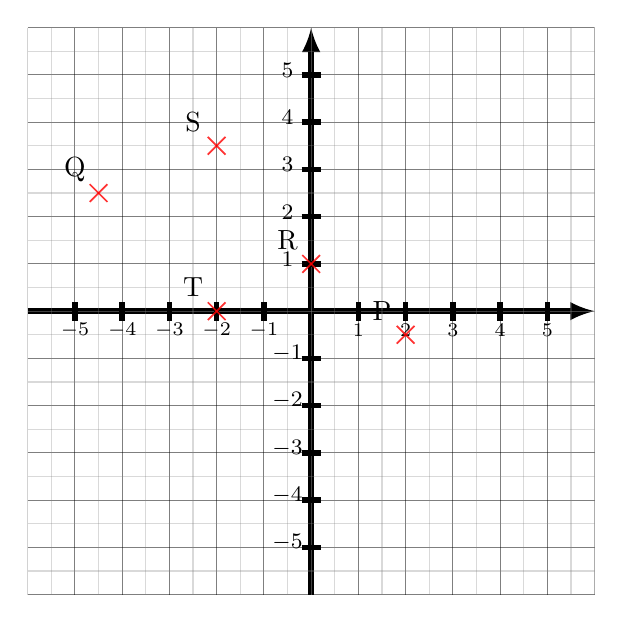
\begin{tikzpicture}[baseline,scale = 0.60]

    \tikzset{
      point/.style={
        thick,
        draw,
        cross out,
        inner sep=0pt,
        minimum width=5pt,
        minimum height=5pt,
      },
    }
    \clip (-6,-6) rectangle (6,6);
    	
	\draw[color ={black},line width = 2,>=latex,->] (-6,0)--(6,0);
	\draw[color ={black},line width = 2,>=latex,->] (0,-6)--(0,6);
	\draw[color ={black},opacity = 0.5] (-6,1)--(6,1);
	\draw[color ={black},opacity = 0.5] (-6,2)--(6,2);
	\draw[color ={black},opacity = 0.5] (-6,3)--(6,3);
	\draw[color ={black},opacity = 0.5] (-6,4)--(6,4);
	\draw[color ={black},opacity = 0.5] (-6,5)--(6,5);
	\draw[color ={black},opacity = 0.5] (-6,6)--(6,6);
	\draw[color ={black},opacity = 0.5] (-6,-1)--(6,-1);
	\draw[color ={black},opacity = 0.5] (-6,-2)--(6,-2);
	\draw[color ={black},opacity = 0.5] (-6,-3)--(6,-3);
	\draw[color ={black},opacity = 0.5] (-6,-4)--(6,-4);
	\draw[color ={black},opacity = 0.5] (-6,-5)--(6,-5);
	\draw[color ={black},opacity = 0.5] (-6,-6)--(6,-6);
	\draw[color ={black},opacity = 0.5] (1,-6)--(1,6);
	\draw[color ={black},opacity = 0.5] (2,-6)--(2,6);
	\draw[color ={black},opacity = 0.5] (3,-6)--(3,6);
	\draw[color ={black},opacity = 0.5] (4,-6)--(4,6);
	\draw[color ={black},opacity = 0.5] (5,-6)--(5,6);
	\draw[color ={black},opacity = 0.5] (6,-6)--(6,6);
	\draw[color ={black},opacity = 0.5] (-1,-6)--(-1,6);
	\draw[color ={black},opacity = 0.5] (-2,-6)--(-2,6);
	\draw[color ={black},opacity = 0.5] (-3,-6)--(-3,6);
	\draw[color ={black},opacity = 0.5] (-4,-6)--(-4,6);
	\draw[color ={black},opacity = 0.5] (-5,-6)--(-5,6);
	\draw[color ={black},opacity = 0.5] (-6,-6)--(-6,6);
	\draw[color ={gray},opacity = 0.3] (-6,0)--(6,0);
	\draw[color ={gray},opacity = 0.3] (-6,0.5)--(6,0.5);
	\draw[color ={gray},opacity = 0.3] (-6,1.5)--(6,1.5);
	\draw[color ={gray},opacity = 0.3] (-6,2.5)--(6,2.5);
	\draw[color ={gray},opacity = 0.3] (-6,3.5)--(6,3.5);
	\draw[color ={gray},opacity = 0.3] (-6,4.5)--(6,4.5);
	\draw[color ={gray},opacity = 0.3] (-6,5.5)--(6,5.5);
	\draw[color ={gray},opacity = 0.3] (-6,0)--(6,0);
	\draw[color ={gray},opacity = 0.3] (-6,-0.5)--(6,-0.5);
	\draw[color ={gray},opacity = 0.3] (-6,-1.5)--(6,-1.5);
	\draw[color ={gray},opacity = 0.3] (-6,-2.5)--(6,-2.5);
	\draw[color ={gray},opacity = 0.3] (-6,-3.5)--(6,-3.5);
	\draw[color ={gray},opacity = 0.3] (-6,-4.5)--(6,-4.5);
	\draw[color ={gray},opacity = 0.3] (-6,-5.5)--(6,-5.5);
	\draw[color ={gray},opacity = 0.3] (0,-6)--(0,6);
	\draw[color ={gray},opacity = 0.3] (0.5,-6)--(0.5,6);
	\draw[color ={gray},opacity = 0.3] (1.5,-6)--(1.5,6);
	\draw[color ={gray},opacity = 0.3] (2.5,-6)--(2.5,6);
	\draw[color ={gray},opacity = 0.3] (3.5,-6)--(3.5,6);
	\draw[color ={gray},opacity = 0.3] (4.5,-6)--(4.5,6);
	\draw[color ={gray},opacity = 0.3] (5.5,-6)--(5.5,6);
	\draw[color ={gray},opacity = 0.3] (0,-6)--(0,6);
	\draw[color ={gray},opacity = 0.3] (-0.5,-6)--(-0.5,6);
	\draw[color ={gray},opacity = 0.3] (-1.5,-6)--(-1.5,6);
	\draw[color ={gray},opacity = 0.3] (-2.5,-6)--(-2.5,6);
	\draw[color ={gray},opacity = 0.3] (-3.5,-6)--(-3.5,6);
	\draw[color ={gray},opacity = 0.3] (-4.5,-6)--(-4.5,6);
	\draw[color ={gray},opacity = 0.3] (-5.5,-6)--(-5.5,6);
	\draw[color ={black},line width = 2] (1,-0.2)--(1,0.2);
	\draw[color ={black},line width = 2] (2,-0.2)--(2,0.2);
	\draw[color ={black},line width = 2] (3,-0.2)--(3,0.2);
	\draw[color ={black},line width = 2] (4,-0.2)--(4,0.2);
	\draw[color ={black},line width = 2] (5,-0.2)--(5,0.2);
	\draw[color ={black},line width = 2] (-1,-0.2)--(-1,0.2);
	\draw[color ={black},line width = 2] (-2,-0.2)--(-2,0.2);
	\draw[color ={black},line width = 2] (-3,-0.2)--(-3,0.2);
	\draw[color ={black},line width = 2] (-4,-0.2)--(-4,0.2);
	\draw[color ={black},line width = 2] (-5,-0.2)--(-5,0.2);
	\draw[color ={black},line width = 2] (-0.2,1)--(0.2,1);
	\draw[color ={black},line width = 2] (-0.2,2)--(0.2,2);
	\draw[color ={black},line width = 2] (-0.2,3)--(0.2,3);
	\draw[color ={black},line width = 2] (-0.2,4)--(0.2,4);
	\draw[color ={black},line width = 2] (-0.2,5)--(0.2,5);
	\draw[color ={black},line width = 2] (-0.2,-1)--(0.2,-1);
	\draw[color ={black},line width = 2] (-0.2,-2)--(0.2,-2);
	\draw[color ={black},line width = 2] (-0.2,-3)--(0.2,-3);
	\draw[color ={black},line width = 2] (-0.2,-4)--(0.2,-4);
	\draw[color ={black},line width = 2] (-0.2,-5)--(0.2,-5);
	\draw (1,-0.4) node[anchor = center] {\scriptsize \color{black}{$1$}};
	\draw (2,-0.4) node[anchor = center] {\scriptsize \color{black}{$2$}};
	\draw (3,-0.4) node[anchor = center] {\scriptsize \color{black}{$3$}};
	\draw (4,-0.4) node[anchor = center] {\scriptsize \color{black}{$4$}};
	\draw (5,-0.4) node[anchor = center] {\scriptsize \color{black}{$5$}};
	\draw (-1,-0.4) node[anchor = center] {\scriptsize \color{black}{$-1$}};
	\draw (-2,-0.4) node[anchor = center] {\scriptsize \color{black}{$-2$}};
	\draw (-3,-0.4) node[anchor = center] {\scriptsize \color{black}{$-3$}};
	\draw (-4,-0.4) node[anchor = center] {\scriptsize \color{black}{$-4$}};
	\draw (-5,-0.4) node[anchor = center] {\scriptsize \color{black}{$-5$}};
	\draw (-0.5,1.1) node[anchor = center] {\footnotesize \color{black}{$1$}};
	\draw (-0.5,2.1) node[anchor = center] {\footnotesize \color{black}{$2$}};
	\draw (-0.5,3.1) node[anchor = center] {\footnotesize \color{black}{$3$}};
	\draw (-0.5,4.1) node[anchor = center] {\footnotesize \color{black}{$4$}};
	\draw (-0.5,5.1) node[anchor = center] {\footnotesize \color{black}{$5$}};
	\draw (-0.5,-0.9) node[anchor = center] {\footnotesize \color{black}{$-1$}};
	\draw (-0.5,-1.9) node[anchor = center] {\footnotesize \color{black}{$-2$}};
	\draw (-0.5,-2.9) node[anchor = center] {\footnotesize \color{black}{$-3$}};
	\draw (-0.5,-3.9) node[anchor = center] {\footnotesize \color{black}{$-4$}};
	\draw (-0.5,-4.9) node[anchor = center] {\footnotesize \color{black}{$-5$}};
	\draw[color ={{red}},line width = 0.625,opacity = 0.8] (1.8125,-0.3125)--(2.1875,-0.6875);\draw[color ={{red}},line width = 0.625,opacity = 0.8] (1.8125,-0.6875)--(2.1875,-0.3125);
	\draw [color={black}] (1.5,0) node[anchor = center,scale=1, rotate = 0] {P};
	\draw[color ={{red}},line width = 0.625,opacity = 0.8] (-2.1875,0.1875)--(-1.8125,-0.1875);\draw[color ={{red}},line width = 0.625,opacity = 0.8] (-2.1875,-0.1875)--(-1.8125,0.1875);
	\draw [color={black}] (-2.5,0.5) node[anchor = center,scale=1, rotate = 0] {T};
	\draw[color ={{red}},line width = 0.625,opacity = 0.8] (-0.1875,1.1875)--(0.1875,0.8125);\draw[color ={{red}},line width = 0.625,opacity = 0.8] (-0.1875,0.8125)--(0.1875,1.1875);
	\draw [color={black}] (-0.5,1.5) node[anchor = center,scale=1, rotate = 0] {R};
	\draw[color ={{red}},line width = 0.625,opacity = 0.8] (-4.6875,2.6875)--(-4.3125,2.3125);\draw[color ={{red}},line width = 0.625,opacity = 0.8] (-4.6875,2.3125)--(-4.3125,2.6875);
	\draw [color={black}] (-5,3) node[anchor = center,scale=1, rotate = 0] {Q};
	\draw[color ={{red}},line width = 0.625,opacity = 0.8] (-2.1875,3.6875)--(-1.8125,3.3125);\draw[color ={{red}},line width = 0.625,opacity = 0.8] (-2.1875,3.3125)--(-1.8125,3.6875);
	\draw [color={black}] (-2.5,4) node[anchor = center,scale=1, rotate = 0] {S};

\end{tikzpicture}\\ \end{minipage}
\end{multicols}
\end{exercice}

\newpage

\begin{multicols}{2}
\begin{exercice}[1]
Placer les points suivants dans le repère : $A(6;-1)$ ;
$B(0;3)$ ; $C(2;0)$ et $D(-4;-5)$.
\medskip
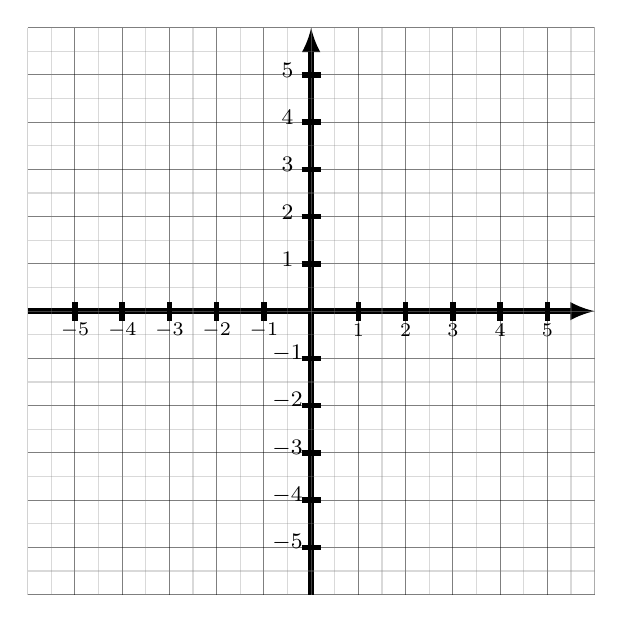
\begin{tikzpicture}[baseline,scale = 0.60]

    \tikzset{
      point/.style={
        thick,
        draw,
        cross out,
        inner sep=0pt,
        minimum width=5pt,
        minimum height=5pt,
      },
    }
    \clip (-6,-6) rectangle (6,6);
    	
	\draw[color ={black},line width = 2,>=latex,->] (-6,0)--(6,0);
	\draw[color ={black},line width = 2,>=latex,->] (0,-6)--(0,6);
	\draw[color ={black},opacity = 0.5] (-6,1)--(6,1);
	\draw[color ={black},opacity = 0.5] (-6,2)--(6,2);
	\draw[color ={black},opacity = 0.5] (-6,3)--(6,3);
	\draw[color ={black},opacity = 0.5] (-6,4)--(6,4);
	\draw[color ={black},opacity = 0.5] (-6,5)--(6,5);
	\draw[color ={black},opacity = 0.5] (-6,6)--(6,6);
	\draw[color ={black},opacity = 0.5] (-6,-1)--(6,-1);
	\draw[color ={black},opacity = 0.5] (-6,-2)--(6,-2);
	\draw[color ={black},opacity = 0.5] (-6,-3)--(6,-3);
	\draw[color ={black},opacity = 0.5] (-6,-4)--(6,-4);
	\draw[color ={black},opacity = 0.5] (-6,-5)--(6,-5);
	\draw[color ={black},opacity = 0.5] (-6,-6)--(6,-6);
	\draw[color ={black},opacity = 0.5] (1,-6)--(1,6);
	\draw[color ={black},opacity = 0.5] (2,-6)--(2,6);
	\draw[color ={black},opacity = 0.5] (3,-6)--(3,6);
	\draw[color ={black},opacity = 0.5] (4,-6)--(4,6);
	\draw[color ={black},opacity = 0.5] (5,-6)--(5,6);
	\draw[color ={black},opacity = 0.5] (6,-6)--(6,6);
	\draw[color ={black},opacity = 0.5] (-1,-6)--(-1,6);
	\draw[color ={black},opacity = 0.5] (-2,-6)--(-2,6);
	\draw[color ={black},opacity = 0.5] (-3,-6)--(-3,6);
	\draw[color ={black},opacity = 0.5] (-4,-6)--(-4,6);
	\draw[color ={black},opacity = 0.5] (-5,-6)--(-5,6);
	\draw[color ={black},opacity = 0.5] (-6,-6)--(-6,6);
	\draw[color ={gray},opacity = 0.3] (-6,0)--(6,0);
	\draw[color ={gray},opacity = 0.3] (-6,0.5)--(6,0.5);
	\draw[color ={gray},opacity = 0.3] (-6,1.5)--(6,1.5);
	\draw[color ={gray},opacity = 0.3] (-6,2.5)--(6,2.5);
	\draw[color ={gray},opacity = 0.3] (-6,3.5)--(6,3.5);
	\draw[color ={gray},opacity = 0.3] (-6,4.5)--(6,4.5);
	\draw[color ={gray},opacity = 0.3] (-6,5.5)--(6,5.5);
	\draw[color ={gray},opacity = 0.3] (-6,0)--(6,0);
	\draw[color ={gray},opacity = 0.3] (-6,-0.5)--(6,-0.5);
	\draw[color ={gray},opacity = 0.3] (-6,-1.5)--(6,-1.5);
	\draw[color ={gray},opacity = 0.3] (-6,-2.5)--(6,-2.5);
	\draw[color ={gray},opacity = 0.3] (-6,-3.5)--(6,-3.5);
	\draw[color ={gray},opacity = 0.3] (-6,-4.5)--(6,-4.5);
	\draw[color ={gray},opacity = 0.3] (-6,-5.5)--(6,-5.5);
	\draw[color ={gray},opacity = 0.3] (0,-6)--(0,6);
	\draw[color ={gray},opacity = 0.3] (0.5,-6)--(0.5,6);
	\draw[color ={gray},opacity = 0.3] (1.5,-6)--(1.5,6);
	\draw[color ={gray},opacity = 0.3] (2.5,-6)--(2.5,6);
	\draw[color ={gray},opacity = 0.3] (3.5,-6)--(3.5,6);
	\draw[color ={gray},opacity = 0.3] (4.5,-6)--(4.5,6);
	\draw[color ={gray},opacity = 0.3] (5.5,-6)--(5.5,6);
	\draw[color ={gray},opacity = 0.3] (0,-6)--(0,6);
	\draw[color ={gray},opacity = 0.3] (-0.5,-6)--(-0.5,6);
	\draw[color ={gray},opacity = 0.3] (-1.5,-6)--(-1.5,6);
	\draw[color ={gray},opacity = 0.3] (-2.5,-6)--(-2.5,6);
	\draw[color ={gray},opacity = 0.3] (-3.5,-6)--(-3.5,6);
	\draw[color ={gray},opacity = 0.3] (-4.5,-6)--(-4.5,6);
	\draw[color ={gray},opacity = 0.3] (-5.5,-6)--(-5.5,6);
	\draw[color ={black},line width = 2] (1,-0.2)--(1,0.2);
	\draw[color ={black},line width = 2] (2,-0.2)--(2,0.2);
	\draw[color ={black},line width = 2] (3,-0.2)--(3,0.2);
	\draw[color ={black},line width = 2] (4,-0.2)--(4,0.2);
	\draw[color ={black},line width = 2] (5,-0.2)--(5,0.2);
	\draw[color ={black},line width = 2] (-1,-0.2)--(-1,0.2);
	\draw[color ={black},line width = 2] (-2,-0.2)--(-2,0.2);
	\draw[color ={black},line width = 2] (-3,-0.2)--(-3,0.2);
	\draw[color ={black},line width = 2] (-4,-0.2)--(-4,0.2);
	\draw[color ={black},line width = 2] (-5,-0.2)--(-5,0.2);
	\draw[color ={black},line width = 2] (-0.2,1)--(0.2,1);
	\draw[color ={black},line width = 2] (-0.2,2)--(0.2,2);
	\draw[color ={black},line width = 2] (-0.2,3)--(0.2,3);
	\draw[color ={black},line width = 2] (-0.2,4)--(0.2,4);
	\draw[color ={black},line width = 2] (-0.2,5)--(0.2,5);
	\draw[color ={black},line width = 2] (-0.2,-1)--(0.2,-1);
	\draw[color ={black},line width = 2] (-0.2,-2)--(0.2,-2);
	\draw[color ={black},line width = 2] (-0.2,-3)--(0.2,-3);
	\draw[color ={black},line width = 2] (-0.2,-4)--(0.2,-4);
	\draw[color ={black},line width = 2] (-0.2,-5)--(0.2,-5);
	\draw (1,-0.4) node[anchor = center] {\scriptsize \color{black}{$1$}};
	\draw (2,-0.4) node[anchor = center] {\scriptsize \color{black}{$2$}};
	\draw (3,-0.4) node[anchor = center] {\scriptsize \color{black}{$3$}};
	\draw (4,-0.4) node[anchor = center] {\scriptsize \color{black}{$4$}};
	\draw (5,-0.4) node[anchor = center] {\scriptsize \color{black}{$5$}};
	\draw (-1,-0.4) node[anchor = center] {\scriptsize \color{black}{$-1$}};
	\draw (-2,-0.4) node[anchor = center] {\scriptsize \color{black}{$-2$}};
	\draw (-3,-0.4) node[anchor = center] {\scriptsize \color{black}{$-3$}};
	\draw (-4,-0.4) node[anchor = center] {\scriptsize \color{black}{$-4$}};
	\draw (-5,-0.4) node[anchor = center] {\scriptsize \color{black}{$-5$}};
	\draw (-0.5,1.1) node[anchor = center] {\footnotesize \color{black}{$1$}};
	\draw (-0.5,2.1) node[anchor = center] {\footnotesize \color{black}{$2$}};
	\draw (-0.5,3.1) node[anchor = center] {\footnotesize \color{black}{$3$}};
	\draw (-0.5,4.1) node[anchor = center] {\footnotesize \color{black}{$4$}};
	\draw (-0.5,5.1) node[anchor = center] {\footnotesize \color{black}{$5$}};
	\draw (-0.5,-0.9) node[anchor = center] {\footnotesize \color{black}{$-1$}};
	\draw (-0.5,-1.9) node[anchor = center] {\footnotesize \color{black}{$-2$}};
	\draw (-0.5,-2.9) node[anchor = center] {\footnotesize \color{black}{$-3$}};
	\draw (-0.5,-3.9) node[anchor = center] {\footnotesize \color{black}{$-4$}};
	\draw (-0.5,-4.9) node[anchor = center] {\footnotesize \color{black}{$-5$}};
	
\end{tikzpicture}
\end{exercice}

\begin{exercice}[1]
Placer les points suivants dans le repère : $E(-5;-1)$ ;
$F(4;4)$ ; $G(-2;-2)$ et $H(-1;-3)$.
\medskip
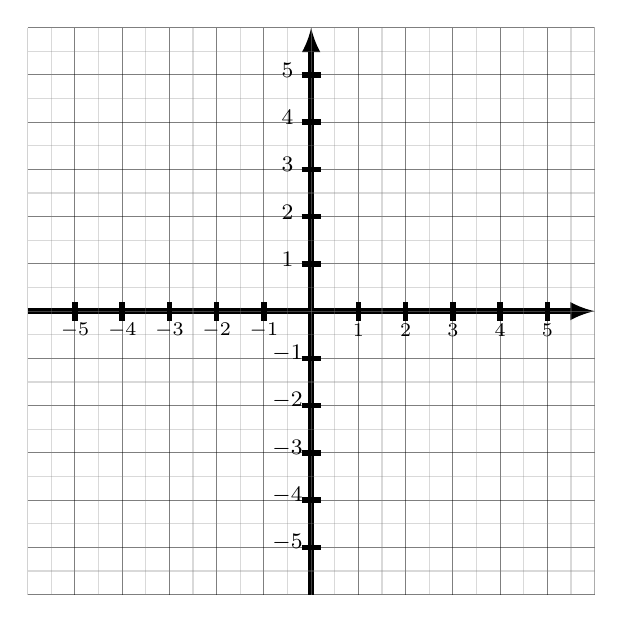
\begin{tikzpicture}[baseline,scale = 0.60]

    \tikzset{
      point/.style={
        thick,
        draw,
        cross out,
        inner sep=0pt,
        minimum width=5pt,
        minimum height=5pt,
      },
    }
    \clip (-6,-6) rectangle (6,6);
    	
	\draw[color ={black},line width = 2,>=latex,->] (-6,0)--(6,0);
	\draw[color ={black},line width = 2,>=latex,->] (0,-6)--(0,6);
	\draw[color ={black},opacity = 0.5] (-6,1)--(6,1);
	\draw[color ={black},opacity = 0.5] (-6,2)--(6,2);
	\draw[color ={black},opacity = 0.5] (-6,3)--(6,3);
	\draw[color ={black},opacity = 0.5] (-6,4)--(6,4);
	\draw[color ={black},opacity = 0.5] (-6,5)--(6,5);
	\draw[color ={black},opacity = 0.5] (-6,6)--(6,6);
	\draw[color ={black},opacity = 0.5] (-6,-1)--(6,-1);
	\draw[color ={black},opacity = 0.5] (-6,-2)--(6,-2);
	\draw[color ={black},opacity = 0.5] (-6,-3)--(6,-3);
	\draw[color ={black},opacity = 0.5] (-6,-4)--(6,-4);
	\draw[color ={black},opacity = 0.5] (-6,-5)--(6,-5);
	\draw[color ={black},opacity = 0.5] (-6,-6)--(6,-6);
	\draw[color ={black},opacity = 0.5] (1,-6)--(1,6);
	\draw[color ={black},opacity = 0.5] (2,-6)--(2,6);
	\draw[color ={black},opacity = 0.5] (3,-6)--(3,6);
	\draw[color ={black},opacity = 0.5] (4,-6)--(4,6);
	\draw[color ={black},opacity = 0.5] (5,-6)--(5,6);
	\draw[color ={black},opacity = 0.5] (6,-6)--(6,6);
	\draw[color ={black},opacity = 0.5] (-1,-6)--(-1,6);
	\draw[color ={black},opacity = 0.5] (-2,-6)--(-2,6);
	\draw[color ={black},opacity = 0.5] (-3,-6)--(-3,6);
	\draw[color ={black},opacity = 0.5] (-4,-6)--(-4,6);
	\draw[color ={black},opacity = 0.5] (-5,-6)--(-5,6);
	\draw[color ={black},opacity = 0.5] (-6,-6)--(-6,6);
	\draw[color ={gray},opacity = 0.3] (-6,0)--(6,0);
	\draw[color ={gray},opacity = 0.3] (-6,0.5)--(6,0.5);
	\draw[color ={gray},opacity = 0.3] (-6,1.5)--(6,1.5);
	\draw[color ={gray},opacity = 0.3] (-6,2.5)--(6,2.5);
	\draw[color ={gray},opacity = 0.3] (-6,3.5)--(6,3.5);
	\draw[color ={gray},opacity = 0.3] (-6,4.5)--(6,4.5);
	\draw[color ={gray},opacity = 0.3] (-6,5.5)--(6,5.5);
	\draw[color ={gray},opacity = 0.3] (-6,0)--(6,0);
	\draw[color ={gray},opacity = 0.3] (-6,-0.5)--(6,-0.5);
	\draw[color ={gray},opacity = 0.3] (-6,-1.5)--(6,-1.5);
	\draw[color ={gray},opacity = 0.3] (-6,-2.5)--(6,-2.5);
	\draw[color ={gray},opacity = 0.3] (-6,-3.5)--(6,-3.5);
	\draw[color ={gray},opacity = 0.3] (-6,-4.5)--(6,-4.5);
	\draw[color ={gray},opacity = 0.3] (-6,-5.5)--(6,-5.5);
	\draw[color ={gray},opacity = 0.3] (0,-6)--(0,6);
	\draw[color ={gray},opacity = 0.3] (0.5,-6)--(0.5,6);
	\draw[color ={gray},opacity = 0.3] (1.5,-6)--(1.5,6);
	\draw[color ={gray},opacity = 0.3] (2.5,-6)--(2.5,6);
	\draw[color ={gray},opacity = 0.3] (3.5,-6)--(3.5,6);
	\draw[color ={gray},opacity = 0.3] (4.5,-6)--(4.5,6);
	\draw[color ={gray},opacity = 0.3] (5.5,-6)--(5.5,6);
	\draw[color ={gray},opacity = 0.3] (0,-6)--(0,6);
	\draw[color ={gray},opacity = 0.3] (-0.5,-6)--(-0.5,6);
	\draw[color ={gray},opacity = 0.3] (-1.5,-6)--(-1.5,6);
	\draw[color ={gray},opacity = 0.3] (-2.5,-6)--(-2.5,6);
	\draw[color ={gray},opacity = 0.3] (-3.5,-6)--(-3.5,6);
	\draw[color ={gray},opacity = 0.3] (-4.5,-6)--(-4.5,6);
	\draw[color ={gray},opacity = 0.3] (-5.5,-6)--(-5.5,6);
	\draw[color ={black},line width = 2] (1,-0.2)--(1,0.2);
	\draw[color ={black},line width = 2] (2,-0.2)--(2,0.2);
	\draw[color ={black},line width = 2] (3,-0.2)--(3,0.2);
	\draw[color ={black},line width = 2] (4,-0.2)--(4,0.2);
	\draw[color ={black},line width = 2] (5,-0.2)--(5,0.2);
	\draw[color ={black},line width = 2] (-1,-0.2)--(-1,0.2);
	\draw[color ={black},line width = 2] (-2,-0.2)--(-2,0.2);
	\draw[color ={black},line width = 2] (-3,-0.2)--(-3,0.2);
	\draw[color ={black},line width = 2] (-4,-0.2)--(-4,0.2);
	\draw[color ={black},line width = 2] (-5,-0.2)--(-5,0.2);
	\draw[color ={black},line width = 2] (-0.2,1)--(0.2,1);
	\draw[color ={black},line width = 2] (-0.2,2)--(0.2,2);
	\draw[color ={black},line width = 2] (-0.2,3)--(0.2,3);
	\draw[color ={black},line width = 2] (-0.2,4)--(0.2,4);
	\draw[color ={black},line width = 2] (-0.2,5)--(0.2,5);
	\draw[color ={black},line width = 2] (-0.2,-1)--(0.2,-1);
	\draw[color ={black},line width = 2] (-0.2,-2)--(0.2,-2);
	\draw[color ={black},line width = 2] (-0.2,-3)--(0.2,-3);
	\draw[color ={black},line width = 2] (-0.2,-4)--(0.2,-4);
	\draw[color ={black},line width = 2] (-0.2,-5)--(0.2,-5);
	\draw (1,-0.4) node[anchor = center] {\scriptsize \color{black}{$1$}};
	\draw (2,-0.4) node[anchor = center] {\scriptsize \color{black}{$2$}};
	\draw (3,-0.4) node[anchor = center] {\scriptsize \color{black}{$3$}};
	\draw (4,-0.4) node[anchor = center] {\scriptsize \color{black}{$4$}};
	\draw (5,-0.4) node[anchor = center] {\scriptsize \color{black}{$5$}};
	\draw (-1,-0.4) node[anchor = center] {\scriptsize \color{black}{$-1$}};
	\draw (-2,-0.4) node[anchor = center] {\scriptsize \color{black}{$-2$}};
	\draw (-3,-0.4) node[anchor = center] {\scriptsize \color{black}{$-3$}};
	\draw (-4,-0.4) node[anchor = center] {\scriptsize \color{black}{$-4$}};
	\draw (-5,-0.4) node[anchor = center] {\scriptsize \color{black}{$-5$}};
	\draw (-0.5,1.1) node[anchor = center] {\footnotesize \color{black}{$1$}};
	\draw (-0.5,2.1) node[anchor = center] {\footnotesize \color{black}{$2$}};
	\draw (-0.5,3.1) node[anchor = center] {\footnotesize \color{black}{$3$}};
	\draw (-0.5,4.1) node[anchor = center] {\footnotesize \color{black}{$4$}};
	\draw (-0.5,5.1) node[anchor = center] {\footnotesize \color{black}{$5$}};
	\draw (-0.5,-0.9) node[anchor = center] {\footnotesize \color{black}{$-1$}};
	\draw (-0.5,-1.9) node[anchor = center] {\footnotesize \color{black}{$-2$}};
	\draw (-0.5,-2.9) node[anchor = center] {\footnotesize \color{black}{$-3$}};
	\draw (-0.5,-3.9) node[anchor = center] {\footnotesize \color{black}{$-4$}};
	\draw (-0.5,-4.9) node[anchor = center] {\footnotesize \color{black}{$-5$}};
	
\end{tikzpicture}

\end{exercice}
\end{multicols}

\begin{multicols}{2}
\begin{exercice}[2]
Placer les points suivants dans le repère : $I(1,5;-1)$ ;
$J(0;-3)$ ; $K(2,5;2,5)$ ; $R(2,5;3)$ et $L(-1,5;-0,5)$.
\medskip
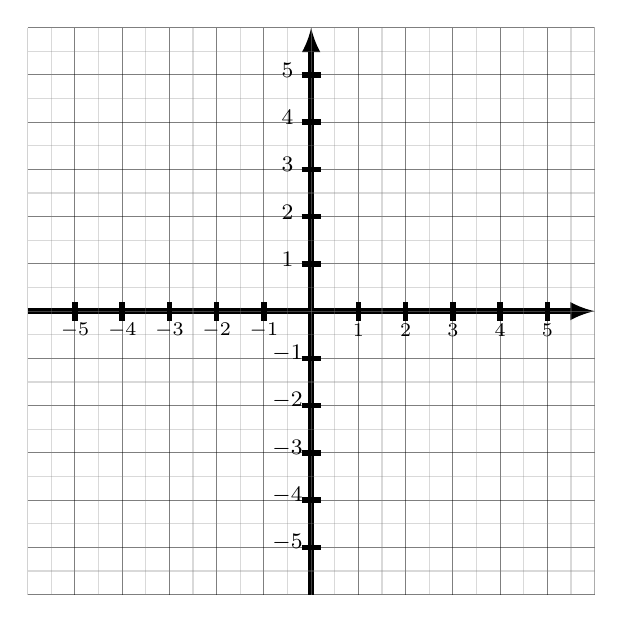
\begin{tikzpicture}[baseline,scale = 0.60]

    \tikzset{
      point/.style={
        thick,
        draw,
        cross out,
        inner sep=0pt,
        minimum width=5pt,
        minimum height=5pt,
      },
    }
    \clip (-6,-6) rectangle (6,6);
    	
	\draw[color ={black},line width = 2,>=latex,->] (-6,0)--(6,0);
	\draw[color ={black},line width = 2,>=latex,->] (0,-6)--(0,6);
	\draw[color ={black},opacity = 0.5] (-6,1)--(6,1);
	\draw[color ={black},opacity = 0.5] (-6,2)--(6,2);
	\draw[color ={black},opacity = 0.5] (-6,3)--(6,3);
	\draw[color ={black},opacity = 0.5] (-6,4)--(6,4);
	\draw[color ={black},opacity = 0.5] (-6,5)--(6,5);
	\draw[color ={black},opacity = 0.5] (-6,6)--(6,6);
	\draw[color ={black},opacity = 0.5] (-6,-1)--(6,-1);
	\draw[color ={black},opacity = 0.5] (-6,-2)--(6,-2);
	\draw[color ={black},opacity = 0.5] (-6,-3)--(6,-3);
	\draw[color ={black},opacity = 0.5] (-6,-4)--(6,-4);
	\draw[color ={black},opacity = 0.5] (-6,-5)--(6,-5);
	\draw[color ={black},opacity = 0.5] (-6,-6)--(6,-6);
	\draw[color ={black},opacity = 0.5] (1,-6)--(1,6);
	\draw[color ={black},opacity = 0.5] (2,-6)--(2,6);
	\draw[color ={black},opacity = 0.5] (3,-6)--(3,6);
	\draw[color ={black},opacity = 0.5] (4,-6)--(4,6);
	\draw[color ={black},opacity = 0.5] (5,-6)--(5,6);
	\draw[color ={black},opacity = 0.5] (6,-6)--(6,6);
	\draw[color ={black},opacity = 0.5] (-1,-6)--(-1,6);
	\draw[color ={black},opacity = 0.5] (-2,-6)--(-2,6);
	\draw[color ={black},opacity = 0.5] (-3,-6)--(-3,6);
	\draw[color ={black},opacity = 0.5] (-4,-6)--(-4,6);
	\draw[color ={black},opacity = 0.5] (-5,-6)--(-5,6);
	\draw[color ={black},opacity = 0.5] (-6,-6)--(-6,6);
	\draw[color ={gray},opacity = 0.3] (-6,0)--(6,0);
	\draw[color ={gray},opacity = 0.3] (-6,0.5)--(6,0.5);
	\draw[color ={gray},opacity = 0.3] (-6,1.5)--(6,1.5);
	\draw[color ={gray},opacity = 0.3] (-6,2.5)--(6,2.5);
	\draw[color ={gray},opacity = 0.3] (-6,3.5)--(6,3.5);
	\draw[color ={gray},opacity = 0.3] (-6,4.5)--(6,4.5);
	\draw[color ={gray},opacity = 0.3] (-6,5.5)--(6,5.5);
	\draw[color ={gray},opacity = 0.3] (-6,0)--(6,0);
	\draw[color ={gray},opacity = 0.3] (-6,-0.5)--(6,-0.5);
	\draw[color ={gray},opacity = 0.3] (-6,-1.5)--(6,-1.5);
	\draw[color ={gray},opacity = 0.3] (-6,-2.5)--(6,-2.5);
	\draw[color ={gray},opacity = 0.3] (-6,-3.5)--(6,-3.5);
	\draw[color ={gray},opacity = 0.3] (-6,-4.5)--(6,-4.5);
	\draw[color ={gray},opacity = 0.3] (-6,-5.5)--(6,-5.5);
	\draw[color ={gray},opacity = 0.3] (0,-6)--(0,6);
	\draw[color ={gray},opacity = 0.3] (0.5,-6)--(0.5,6);
	\draw[color ={gray},opacity = 0.3] (1.5,-6)--(1.5,6);
	\draw[color ={gray},opacity = 0.3] (2.5,-6)--(2.5,6);
	\draw[color ={gray},opacity = 0.3] (3.5,-6)--(3.5,6);
	\draw[color ={gray},opacity = 0.3] (4.5,-6)--(4.5,6);
	\draw[color ={gray},opacity = 0.3] (5.5,-6)--(5.5,6);
	\draw[color ={gray},opacity = 0.3] (0,-6)--(0,6);
	\draw[color ={gray},opacity = 0.3] (-0.5,-6)--(-0.5,6);
	\draw[color ={gray},opacity = 0.3] (-1.5,-6)--(-1.5,6);
	\draw[color ={gray},opacity = 0.3] (-2.5,-6)--(-2.5,6);
	\draw[color ={gray},opacity = 0.3] (-3.5,-6)--(-3.5,6);
	\draw[color ={gray},opacity = 0.3] (-4.5,-6)--(-4.5,6);
	\draw[color ={gray},opacity = 0.3] (-5.5,-6)--(-5.5,6);
	\draw[color ={black},line width = 2] (1,-0.2)--(1,0.2);
	\draw[color ={black},line width = 2] (2,-0.2)--(2,0.2);
	\draw[color ={black},line width = 2] (3,-0.2)--(3,0.2);
	\draw[color ={black},line width = 2] (4,-0.2)--(4,0.2);
	\draw[color ={black},line width = 2] (5,-0.2)--(5,0.2);
	\draw[color ={black},line width = 2] (-1,-0.2)--(-1,0.2);
	\draw[color ={black},line width = 2] (-2,-0.2)--(-2,0.2);
	\draw[color ={black},line width = 2] (-3,-0.2)--(-3,0.2);
	\draw[color ={black},line width = 2] (-4,-0.2)--(-4,0.2);
	\draw[color ={black},line width = 2] (-5,-0.2)--(-5,0.2);
	\draw[color ={black},line width = 2] (-0.2,1)--(0.2,1);
	\draw[color ={black},line width = 2] (-0.2,2)--(0.2,2);
	\draw[color ={black},line width = 2] (-0.2,3)--(0.2,3);
	\draw[color ={black},line width = 2] (-0.2,4)--(0.2,4);
	\draw[color ={black},line width = 2] (-0.2,5)--(0.2,5);
	\draw[color ={black},line width = 2] (-0.2,-1)--(0.2,-1);
	\draw[color ={black},line width = 2] (-0.2,-2)--(0.2,-2);
	\draw[color ={black},line width = 2] (-0.2,-3)--(0.2,-3);
	\draw[color ={black},line width = 2] (-0.2,-4)--(0.2,-4);
	\draw[color ={black},line width = 2] (-0.2,-5)--(0.2,-5);
	\draw (1,-0.4) node[anchor = center] {\scriptsize \color{black}{$1$}};
	\draw (2,-0.4) node[anchor = center] {\scriptsize \color{black}{$2$}};
	\draw (3,-0.4) node[anchor = center] {\scriptsize \color{black}{$3$}};
	\draw (4,-0.4) node[anchor = center] {\scriptsize \color{black}{$4$}};
	\draw (5,-0.4) node[anchor = center] {\scriptsize \color{black}{$5$}};
	\draw (-1,-0.4) node[anchor = center] {\scriptsize \color{black}{$-1$}};
	\draw (-2,-0.4) node[anchor = center] {\scriptsize \color{black}{$-2$}};
	\draw (-3,-0.4) node[anchor = center] {\scriptsize \color{black}{$-3$}};
	\draw (-4,-0.4) node[anchor = center] {\scriptsize \color{black}{$-4$}};
	\draw (-5,-0.4) node[anchor = center] {\scriptsize \color{black}{$-5$}};
	\draw (-0.5,1.1) node[anchor = center] {\footnotesize \color{black}{$1$}};
	\draw (-0.5,2.1) node[anchor = center] {\footnotesize \color{black}{$2$}};
	\draw (-0.5,3.1) node[anchor = center] {\footnotesize \color{black}{$3$}};
	\draw (-0.5,4.1) node[anchor = center] {\footnotesize \color{black}{$4$}};
	\draw (-0.5,5.1) node[anchor = center] {\footnotesize \color{black}{$5$}};
	\draw (-0.5,-0.9) node[anchor = center] {\footnotesize \color{black}{$-1$}};
	\draw (-0.5,-1.9) node[anchor = center] {\footnotesize \color{black}{$-2$}};
	\draw (-0.5,-2.9) node[anchor = center] {\footnotesize \color{black}{$-3$}};
	\draw (-0.5,-3.9) node[anchor = center] {\footnotesize \color{black}{$-4$}};
	\draw (-0.5,-4.9) node[anchor = center] {\footnotesize \color{black}{$-5$}};
	
\end{tikzpicture}
\end{exercice}



\begin{exercice}[2]
Placer les points suivants dans le repère : $M(-4,5;-2,5)$ ;
$N(0,5;2,5)$ ; $O(1,5;-0,5)$, $P(-4,5;-3,5)$ et $Q(-1,5;1,5)$.
\medskip
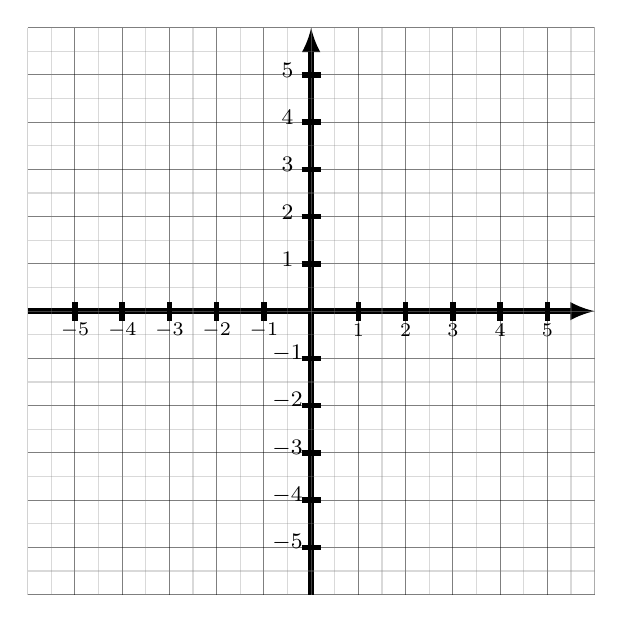
\begin{tikzpicture}[baseline,scale = 0.60]

    \tikzset{
      point/.style={
        thick,
        draw,
        cross out,
        inner sep=0pt,
        minimum width=5pt,
        minimum height=5pt,
      },
    }
    \clip (-6,-6) rectangle (6,6);
    	
	\draw[color ={black},line width = 2,>=latex,->] (-6,0)--(6,0);
	\draw[color ={black},line width = 2,>=latex,->] (0,-6)--(0,6);
	\draw[color ={black},opacity = 0.5] (-6,1)--(6,1);
	\draw[color ={black},opacity = 0.5] (-6,2)--(6,2);
	\draw[color ={black},opacity = 0.5] (-6,3)--(6,3);
	\draw[color ={black},opacity = 0.5] (-6,4)--(6,4);
	\draw[color ={black},opacity = 0.5] (-6,5)--(6,5);
	\draw[color ={black},opacity = 0.5] (-6,6)--(6,6);
	\draw[color ={black},opacity = 0.5] (-6,-1)--(6,-1);
	\draw[color ={black},opacity = 0.5] (-6,-2)--(6,-2);
	\draw[color ={black},opacity = 0.5] (-6,-3)--(6,-3);
	\draw[color ={black},opacity = 0.5] (-6,-4)--(6,-4);
	\draw[color ={black},opacity = 0.5] (-6,-5)--(6,-5);
	\draw[color ={black},opacity = 0.5] (-6,-6)--(6,-6);
	\draw[color ={black},opacity = 0.5] (1,-6)--(1,6);
	\draw[color ={black},opacity = 0.5] (2,-6)--(2,6);
	\draw[color ={black},opacity = 0.5] (3,-6)--(3,6);
	\draw[color ={black},opacity = 0.5] (4,-6)--(4,6);
	\draw[color ={black},opacity = 0.5] (5,-6)--(5,6);
	\draw[color ={black},opacity = 0.5] (6,-6)--(6,6);
	\draw[color ={black},opacity = 0.5] (-1,-6)--(-1,6);
	\draw[color ={black},opacity = 0.5] (-2,-6)--(-2,6);
	\draw[color ={black},opacity = 0.5] (-3,-6)--(-3,6);
	\draw[color ={black},opacity = 0.5] (-4,-6)--(-4,6);
	\draw[color ={black},opacity = 0.5] (-5,-6)--(-5,6);
	\draw[color ={black},opacity = 0.5] (-6,-6)--(-6,6);
	\draw[color ={gray},opacity = 0.3] (-6,0)--(6,0);
	\draw[color ={gray},opacity = 0.3] (-6,0.5)--(6,0.5);
	\draw[color ={gray},opacity = 0.3] (-6,1.5)--(6,1.5);
	\draw[color ={gray},opacity = 0.3] (-6,2.5)--(6,2.5);
	\draw[color ={gray},opacity = 0.3] (-6,3.5)--(6,3.5);
	\draw[color ={gray},opacity = 0.3] (-6,4.5)--(6,4.5);
	\draw[color ={gray},opacity = 0.3] (-6,5.5)--(6,5.5);
	\draw[color ={gray},opacity = 0.3] (-6,0)--(6,0);
	\draw[color ={gray},opacity = 0.3] (-6,-0.5)--(6,-0.5);
	\draw[color ={gray},opacity = 0.3] (-6,-1.5)--(6,-1.5);
	\draw[color ={gray},opacity = 0.3] (-6,-2.5)--(6,-2.5);
	\draw[color ={gray},opacity = 0.3] (-6,-3.5)--(6,-3.5);
	\draw[color ={gray},opacity = 0.3] (-6,-4.5)--(6,-4.5);
	\draw[color ={gray},opacity = 0.3] (-6,-5.5)--(6,-5.5);
	\draw[color ={gray},opacity = 0.3] (0,-6)--(0,6);
	\draw[color ={gray},opacity = 0.3] (0.5,-6)--(0.5,6);
	\draw[color ={gray},opacity = 0.3] (1.5,-6)--(1.5,6);
	\draw[color ={gray},opacity = 0.3] (2.5,-6)--(2.5,6);
	\draw[color ={gray},opacity = 0.3] (3.5,-6)--(3.5,6);
	\draw[color ={gray},opacity = 0.3] (4.5,-6)--(4.5,6);
	\draw[color ={gray},opacity = 0.3] (5.5,-6)--(5.5,6);
	\draw[color ={gray},opacity = 0.3] (0,-6)--(0,6);
	\draw[color ={gray},opacity = 0.3] (-0.5,-6)--(-0.5,6);
	\draw[color ={gray},opacity = 0.3] (-1.5,-6)--(-1.5,6);
	\draw[color ={gray},opacity = 0.3] (-2.5,-6)--(-2.5,6);
	\draw[color ={gray},opacity = 0.3] (-3.5,-6)--(-3.5,6);
	\draw[color ={gray},opacity = 0.3] (-4.5,-6)--(-4.5,6);
	\draw[color ={gray},opacity = 0.3] (-5.5,-6)--(-5.5,6);
	\draw[color ={black},line width = 2] (1,-0.2)--(1,0.2);
	\draw[color ={black},line width = 2] (2,-0.2)--(2,0.2);
	\draw[color ={black},line width = 2] (3,-0.2)--(3,0.2);
	\draw[color ={black},line width = 2] (4,-0.2)--(4,0.2);
	\draw[color ={black},line width = 2] (5,-0.2)--(5,0.2);
	\draw[color ={black},line width = 2] (-1,-0.2)--(-1,0.2);
	\draw[color ={black},line width = 2] (-2,-0.2)--(-2,0.2);
	\draw[color ={black},line width = 2] (-3,-0.2)--(-3,0.2);
	\draw[color ={black},line width = 2] (-4,-0.2)--(-4,0.2);
	\draw[color ={black},line width = 2] (-5,-0.2)--(-5,0.2);
	\draw[color ={black},line width = 2] (-0.2,1)--(0.2,1);
	\draw[color ={black},line width = 2] (-0.2,2)--(0.2,2);
	\draw[color ={black},line width = 2] (-0.2,3)--(0.2,3);
	\draw[color ={black},line width = 2] (-0.2,4)--(0.2,4);
	\draw[color ={black},line width = 2] (-0.2,5)--(0.2,5);
	\draw[color ={black},line width = 2] (-0.2,-1)--(0.2,-1);
	\draw[color ={black},line width = 2] (-0.2,-2)--(0.2,-2);
	\draw[color ={black},line width = 2] (-0.2,-3)--(0.2,-3);
	\draw[color ={black},line width = 2] (-0.2,-4)--(0.2,-4);
	\draw[color ={black},line width = 2] (-0.2,-5)--(0.2,-5);
	\draw (1,-0.4) node[anchor = center] {\scriptsize \color{black}{$1$}};
	\draw (2,-0.4) node[anchor = center] {\scriptsize \color{black}{$2$}};
	\draw (3,-0.4) node[anchor = center] {\scriptsize \color{black}{$3$}};
	\draw (4,-0.4) node[anchor = center] {\scriptsize \color{black}{$4$}};
	\draw (5,-0.4) node[anchor = center] {\scriptsize \color{black}{$5$}};
	\draw (-1,-0.4) node[anchor = center] {\scriptsize \color{black}{$-1$}};
	\draw (-2,-0.4) node[anchor = center] {\scriptsize \color{black}{$-2$}};
	\draw (-3,-0.4) node[anchor = center] {\scriptsize \color{black}{$-3$}};
	\draw (-4,-0.4) node[anchor = center] {\scriptsize \color{black}{$-4$}};
	\draw (-5,-0.4) node[anchor = center] {\scriptsize \color{black}{$-5$}};
	\draw (-0.5,1.1) node[anchor = center] {\footnotesize \color{black}{$1$}};
	\draw (-0.5,2.1) node[anchor = center] {\footnotesize \color{black}{$2$}};
	\draw (-0.5,3.1) node[anchor = center] {\footnotesize \color{black}{$3$}};
	\draw (-0.5,4.1) node[anchor = center] {\footnotesize \color{black}{$4$}};
	\draw (-0.5,5.1) node[anchor = center] {\footnotesize \color{black}{$5$}};
	\draw (-0.5,-0.9) node[anchor = center] {\footnotesize \color{black}{$-1$}};
	\draw (-0.5,-1.9) node[anchor = center] {\footnotesize \color{black}{$-2$}};
	\draw (-0.5,-2.9) node[anchor = center] {\footnotesize \color{black}{$-3$}};
	\draw (-0.5,-3.9) node[anchor = center] {\footnotesize \color{black}{$-4$}};
	\draw (-0.5,-4.9) node[anchor = center] {\footnotesize \color{black}{$-5$}};
	
\end{tikzpicture}
\end{exercice}
\end{multicols}

\end{document}
